% Options for packages loaded elsewhere
\PassOptionsToPackage{unicode}{hyperref}
\PassOptionsToPackage{hyphens}{url}
\PassOptionsToPackage{dvipsnames,svgnames,x11names}{xcolor}
%
\documentclass[
  letterpaper,
  DIV=11,
  numbers=noendperiod]{scrartcl}

\usepackage{amsmath,amssymb}
\usepackage{lmodern}
\usepackage{iftex}
\ifPDFTeX
  \usepackage[T1]{fontenc}
  \usepackage[utf8]{inputenc}
  \usepackage{textcomp} % provide euro and other symbols
\else % if luatex or xetex
  \usepackage{unicode-math}
  \defaultfontfeatures{Scale=MatchLowercase}
  \defaultfontfeatures[\rmfamily]{Ligatures=TeX,Scale=1}
\fi
% Use upquote if available, for straight quotes in verbatim environments
\IfFileExists{upquote.sty}{\usepackage{upquote}}{}
\IfFileExists{microtype.sty}{% use microtype if available
  \usepackage[]{microtype}
  \UseMicrotypeSet[protrusion]{basicmath} % disable protrusion for tt fonts
}{}
\makeatletter
\@ifundefined{KOMAClassName}{% if non-KOMA class
  \IfFileExists{parskip.sty}{%
    \usepackage{parskip}
  }{% else
    \setlength{\parindent}{0pt}
    \setlength{\parskip}{6pt plus 2pt minus 1pt}}
}{% if KOMA class
  \KOMAoptions{parskip=half}}
\makeatother
\usepackage{xcolor}
\setlength{\emergencystretch}{3em} % prevent overfull lines
\setcounter{secnumdepth}{5}
% Make \paragraph and \subparagraph free-standing
\ifx\paragraph\undefined\else
  \let\oldparagraph\paragraph
  \renewcommand{\paragraph}[1]{\oldparagraph{#1}\mbox{}}
\fi
\ifx\subparagraph\undefined\else
  \let\oldsubparagraph\subparagraph
  \renewcommand{\subparagraph}[1]{\oldsubparagraph{#1}\mbox{}}
\fi


\providecommand{\tightlist}{%
  \setlength{\itemsep}{0pt}\setlength{\parskip}{0pt}}\usepackage{longtable,booktabs,array}
\usepackage{calc} % for calculating minipage widths
% Correct order of tables after \paragraph or \subparagraph
\usepackage{etoolbox}
\makeatletter
\patchcmd\longtable{\par}{\if@noskipsec\mbox{}\fi\par}{}{}
\makeatother
% Allow footnotes in longtable head/foot
\IfFileExists{footnotehyper.sty}{\usepackage{footnotehyper}}{\usepackage{footnote}}
\makesavenoteenv{longtable}
\usepackage{graphicx}
\makeatletter
\def\maxwidth{\ifdim\Gin@nat@width>\linewidth\linewidth\else\Gin@nat@width\fi}
\def\maxheight{\ifdim\Gin@nat@height>\textheight\textheight\else\Gin@nat@height\fi}
\makeatother
% Scale images if necessary, so that they will not overflow the page
% margins by default, and it is still possible to overwrite the defaults
% using explicit options in \includegraphics[width, height, ...]{}
\setkeys{Gin}{width=\maxwidth,height=\maxheight,keepaspectratio}
% Set default figure placement to htbp
\makeatletter
\def\fps@figure{htbp}
\makeatother
\newlength{\cslhangindent}
\setlength{\cslhangindent}{1.5em}
\newlength{\csllabelwidth}
\setlength{\csllabelwidth}{3em}
\newlength{\cslentryspacingunit} % times entry-spacing
\setlength{\cslentryspacingunit}{\parskip}
\newenvironment{CSLReferences}[2] % #1 hanging-ident, #2 entry spacing
 {% don't indent paragraphs
  \setlength{\parindent}{0pt}
  % turn on hanging indent if param 1 is 1
  \ifodd #1
  \let\oldpar\par
  \def\par{\hangindent=\cslhangindent\oldpar}
  \fi
  % set entry spacing
  \setlength{\parskip}{#2\cslentryspacingunit}
 }%
 {}
\usepackage{calc}
\newcommand{\CSLBlock}[1]{#1\hfill\break}
\newcommand{\CSLLeftMargin}[1]{\parbox[t]{\csllabelwidth}{#1}}
\newcommand{\CSLRightInline}[1]{\parbox[t]{\linewidth - \csllabelwidth}{#1}\break}
\newcommand{\CSLIndent}[1]{\hspace{\cslhangindent}#1}

\usepackage{booktabs}
\usepackage{longtable}
\usepackage{array}
\usepackage{multirow}
\usepackage{wrapfig}
\usepackage{float}
\usepackage{colortbl}
\usepackage{pdflscape}
\usepackage{tabu}
\usepackage{threeparttable}
\usepackage{threeparttablex}
\usepackage[normalem]{ulem}
\usepackage{makecell}
\usepackage{xcolor}
\usepackage{fontspec}
\usepackage{multicol}
\usepackage{hhline}
\usepackage{hyperref}
\usepackage{placeins}
\KOMAoption{captions}{tableheading}
\makeatletter
\makeatother
\makeatletter
\makeatother
\makeatletter
\@ifpackageloaded{caption}{}{\usepackage{caption}}
\AtBeginDocument{%
\ifdefined\contentsname
  \renewcommand*\contentsname{Table of contents}
\else
  \newcommand\contentsname{Table of contents}
\fi
\ifdefined\listfigurename
  \renewcommand*\listfigurename{List of Figures}
\else
  \newcommand\listfigurename{List of Figures}
\fi
\ifdefined\listtablename
  \renewcommand*\listtablename{List of Tables}
\else
  \newcommand\listtablename{List of Tables}
\fi
\ifdefined\figurename
  \renewcommand*\figurename{Figure}
\else
  \newcommand\figurename{Figure}
\fi
\ifdefined\tablename
  \renewcommand*\tablename{Table}
\else
  \newcommand\tablename{Table}
\fi
}
\@ifpackageloaded{float}{}{\usepackage{float}}
\floatstyle{ruled}
\@ifundefined{c@chapter}{\newfloat{codelisting}{h}{lop}}{\newfloat{codelisting}{h}{lop}[chapter]}
\floatname{codelisting}{Listing}
\newcommand*\listoflistings{\listof{codelisting}{List of Listings}}
\makeatother
\makeatletter
\@ifpackageloaded{caption}{}{\usepackage{caption}}
\@ifpackageloaded{subcaption}{}{\usepackage{subcaption}}
\makeatother
\makeatletter
\@ifpackageloaded{tcolorbox}{}{\usepackage[many]{tcolorbox}}
\makeatother
\makeatletter
\@ifundefined{shadecolor}{\definecolor{shadecolor}{rgb}{.97, .97, .97}}
\makeatother
\makeatletter
\makeatother
\ifLuaTeX
  \usepackage{selnolig}  % disable illegal ligatures
\fi
\IfFileExists{bookmark.sty}{\usepackage{bookmark}}{\usepackage{hyperref}}
\IfFileExists{xurl.sty}{\usepackage{xurl}}{} % add URL line breaks if available
\urlstyle{same} % disable monospaced font for URLs
\hypersetup{
  pdftitle={Covid-19 Fields Survey Data Protocol},
  pdfauthor={Ariel Mundo Ortiz},
  colorlinks=true,
  linkcolor={blue},
  filecolor={Maroon},
  citecolor={Blue},
  urlcolor={Blue},
  pdfcreator={LaTeX via pandoc}}

\title{Covid-19 Fields Survey Data Protocol}
\author{Ariel Mundo Ortiz}
\date{1/15/23}

\begin{document}
\maketitle
\ifdefined\Shaded\renewenvironment{Shaded}{\begin{tcolorbox}[borderline west={3pt}{0pt}{shadecolor}, enhanced, boxrule=0pt, breakable, sharp corners, interior hidden, frame hidden]}{\end{tcolorbox}}\fi

\hypertarget{background}{%
\section{Background}\label{background}}

The COVID-19 pandemic continues around the world with more than 600
million confirmed cases as of November of
2022\textsuperscript{\protect\hyperlink{ref-WHO-Covid}{1}}. During the
first months of the pandemic in early 2020, non-pharmaceutical
interventions (e.g., masking, social distancing) were the only methods
available to manage the spread of the disease, but the rapid development
of vaccines against the virus permitted their approval and use in some
countries towards the last month part of 2020. For example, in the US
and Canada vaccine campaigns began in mid-December of
2020\textsuperscript{\protect\hyperlink{ref-tanne2020}{2},\protect\hyperlink{ref-bogoch2022}{3}}.
Although it has been estimated that vaccines against COVID-19 have
prevented around 14 millions of deaths
worldwide\textsuperscript{\protect\hyperlink{ref-watson2022}{4}}, the
rollout of COVID-19 vaccines has faced multiple challenges since its
inception.

In this regard, vaccination efforts have faced multiple: Inequalities
with regard to vaccine access due to socio-economic factors, vaccine
hesitancy, and differences in vaccination rates across different
segments of the population are among the challenges identified in the
administration of COVID-19
vaccines\textsuperscript{\protect\hyperlink{ref-gerretsen2021}{5}--\protect\hyperlink{ref-malik2020}{7}}.
In the case of Canada, lower vaccine uptake has been associated with
socio-economic factors such as younger age, educational level, presence
of children in the household, lack of a regular healthcare provider,
ethnic origin, and financial
instability\textsuperscript{\protect\hyperlink{ref-guay2022}{8}--\protect\hyperlink{ref-carter2022}{10}}.

Additionally, it has been shown that geography also plays a crucial role
in vaccination rates, as they vary due to spatial differences in
attitudes towards
vaccination\textsuperscript{\protect\hyperlink{ref-malik2020}{7}},
geographical differences in vaccine access and supply, vaccination
location availability, and lack of prioritization of vulnerable
groups\textsuperscript{\protect\hyperlink{ref-bogoch2022}{3},\protect\hyperlink{ref-nguyen2021}{11}}.

Studies that analyze geographical variations in vaccine uptake can help
inform public health decision-makers to design policies to that are
aimed at addressing vaccination disparities. In this regard, previous
geographical (spatial) analyses of vaccination rates have shown that
variations in vaccine uptake can occur within small governmental
administrative units (e.g., counties in the case of the
US)\textsuperscript{\protect\hyperlink{ref-mollalo2021}{12}--\protect\hyperlink{ref-bhuiyan2022}{15}},
and that geographical analyses can be predictive of booster uptake
patterns\textsuperscript{\protect\hyperlink{ref-wood2022}{16}}.

In Canada, studies that have used a spatial approach to analyze vaccine
uptake have shown disparities in vaccination rates across low and high
income neighborhoods in the city of
Toronto\textsuperscript{\protect\hyperlink{ref-choi2021}{17}}, among
adolescents from deprived neighborhoods in the city of
Montreal\textsuperscript{\protect\hyperlink{ref-mckinnon2021}{18}}, and
highlighted disparities in vaccination status depending on age, income,
and ethnic origin in all of the Canadian
provinces\textsuperscript{\protect\hyperlink{ref-guay2022}{8}}. However,
to the best of our knowledge, there are no studies that have analyzed
vaccination status within a province to identify inequalities that may
exist within these geographical areas. A dissagregated view of
variability within a province can help understand the barriers for
vaccine delivery in the case of visible minorities, which have been
disproportionately impacted in the
pandemic\textsuperscript{\protect\hyperlink{ref-hussain2022}{19}}.

\hypertarget{research-question}{%
\section{Research Question}\label{research-question}}

This study will examine self-reported COVID-19 vaccination status within
the province of Ontario in order to determine how socio-economic (e.g.,
ethnic origin, age, income) and geographical factors (at level of the
Health Regions of Ontario) influence vaccination within the province.

\hypertarget{methods}{%
\section{Methods}\label{methods}}

\hypertarget{data-source-survey-overview}{%
\subsection{Data source: survey
overview}\label{data-source-survey-overview}}

We obtained data from the Fields Institute for Research in Mathematical
Sciences' (henceforth Fields) \emph{Survey of COVID-19 related
Behaviours and Attitudes}, a repeated cross sectional survey focused on
the Canadian province of Ontario which ran from Sept 30, 2021 until
January 17, 2022. This survey was commissioned by Fields and the
Mathematical Modelling of COVID-19 Task Force, under the supervision of
Dr.~Kumar Murty, the Director of Fields with funding from the Canadian
Institutes of Health Research. The survey was conducted by a third-party
service provider (RIWI Corp.), under ethical guidance from University of
Toronto.

The survey was deployed using random domain intercept technology.
Briefly, when web users clicked on a registered but commercially
inactive web link or typed in a web address for a site that was dormant,
they had a random chance of that link being temporarily managed by the
company that administered the survey (RIWI Corp). Thus, instead of
coming across a notification about the status of the site(``this page
does not exist''), the survey was deployed to the user. Web users then
decided whether to anonymously participate, exiting the survey at any
time if
desired\textsuperscript{\protect\hyperlink{ref-sargent2022}{20}}.

Respondents who wished to participate were asked to select their age
from a matrix of values, and subsequent questions were displayed one at
a time, after the respondent confirmed their selection by answering and
selecting ``next''. Those who do not wished to participate were asked to
either close the browser window or navigate away from the domain. After
the survey closed (complete or incomplete) no one from that internet
protocol (IP) address could access the survey again and the domain entry
point rotated such that if a respondent were to attempt to access the
survey again, share the link, or enter via the same address using an
alternative IP address, the survey would not render.

Additionally, respondents who indicated they were under the age of 16
were exited from the survey. No record was created in this case and due
to domain cycling these users were unable to navigate back to the ``age
select'' screen. The personal identifier information from each
respondent was automatically scrubbed and replaced by a unique ID.
Respondents were drawn exclusively from the province of Ontario, as per
their devices meta-data.

\hypertarget{survey-responses}{%
\subsection{Survey responses}\label{survey-responses}}

\hypertarget{sec-socio-demographic-factors}{%
\subsubsection{Socio-demographic
factors}\label{sec-socio-demographic-factors}}

From the different answers provided by the survey respondents, we
selected the age group which they belonged to, income bracket,
race/ethnicity, and employment status. The original survey included
additional questions (e.g., sick leave, remote work, presence of minors
in the household) but the survey design, which permitted respondents to
exit the survey at any point resulted in a high rates of missing data
for most of these answers. The socio-economic factors chosen for this
study were the ones that had both the lowest rates of missingness and
that provided an adequate level socio-economic and demographic
information for our analysis. Information about the chosen
socio-economic factors from the survey is provided in
Table~\ref{tbl-covariates}.

\hypertarget{tbl-covariates}{}
\begin{longtable}[]{@{}
  >{\raggedright\arraybackslash}p{(\columnwidth - 2\tabcolsep) * \real{0.2361}}
  >{\raggedright\arraybackslash}p{(\columnwidth - 2\tabcolsep) * \real{0.7639}}@{}}
\caption{\label{tbl-covariates}Selected socio-economic factors from the
survey}\tabularnewline
\toprule()
\begin{minipage}[b]{\linewidth}\raggedright
Variable
\end{minipage} & \begin{minipage}[b]{\linewidth}\raggedright
Values
\end{minipage} \\
\midrule()
\endfirsthead
\toprule()
\begin{minipage}[b]{\linewidth}\raggedright
Variable
\end{minipage} & \begin{minipage}[b]{\linewidth}\raggedright
Values
\end{minipage} \\
\midrule()
\endhead
Age group & 15-24,25-34,35-44,45-54,55-64, 65+ \\
Income bracket (CAD) & \textless15,000, 15,000-24,999, 25,000-39,999,
40,000-59,999, 60,000-89,999, \textgreater90,000 \\
Race/ethnicity & Arab/Middle Eastern, Black, East Asian/Pacific
Islander, Indigenous, Latin American, Mixed, South Asian, White
Caucasian, other \\
& \\
\bottomrule()
\end{longtable}

\hypertarget{vaccination-status}{%
\subsubsection{Vaccination status}\label{vaccination-status}}

From the survey, we selected the question regarding vaccination status:

\begin{itemize}
\tightlist
\item
  ``Have you received the first dose of the COVID vaccine?'', with
  possible answers ``yes'' and ``no''
\end{itemize}

\hypertarget{data-cleaning}{%
\subsection{Data cleaning}\label{data-cleaning}}

The original dataset contained 39,029 entries (where each entry
corresponded to a set of answers provided by a unique respondent).
Following a preliminary analysis to identify the missing rates across
the different answers within each entry, it was identified that many of
the answers had high missing rates (\textgreater80\%) (note that the
graph will be in the Appendix). Therefore, the dataset was cleaned in
order to contain only the independent variables of interest with the
lowest missing rates (Table~\ref{tbl-covariates}) and the dependent
variable. The final clean dataset contained 3,709 unique entries.

The cleaning process also included removing outliers that were
identified during the preliminary analyses. Specifically, we removed
those respondents that indicated to be below 25 years of age, living in
a household of size 1, and that reported an income above CAD 110,000.
After cleaning the dataset contained 5,247 entries (unique respondents).

\hypertarget{sec-geographical-location}{%
\subsubsection{Geographical location}\label{sec-geographical-location}}

For each survey participant certain data was automatically captured.
This included the nearest municipality, which resulted in a total of 578
different municipalities within the dataset. Because our interest was to
analyze the differences between Health Regions, we assigned the location
(city) of each entry to its correspondent Health Region following a
multi-step process: First, we used the municipality information from the
website of the Association of Municipalities of Ontario (AMO) to assign
geographical regions to each entry on the dataset. Secondly, we used a
publicly available dataset of long-term care homes by Local Health
Integrated Network (LHIN), which were the geographical divisions for
health in Ontario before the adoption of the Health Regions, to match
each city with its corresponding LHIN. Cities that did not have a LHIN
entry on the dataset were searched in the websites of the LHINs and
manually added to the dataset. Finally, we assigned the corresponding
Health Regio to each city by matching the LHINs to the Health Regions
that now encompass them, following the information provided by Ontario
Health (details of the complete process are in the Appendix).

\hypertarget{corrections}{%
\subsection{Corrections}\label{corrections}}

We identified differences between the proportions of various
socio-economic factors the survey respondents when compared to the 2016
Census data for Ontario. These factors included age groups, income, and
ethnicity/race identified. Additionally, because the Census divisions do
not match the exact boundaries of the Census, we also obtained
population estimates for each Health Region from the Ontario Health
website in order to correct for the population within each Health
Region. We corrected for all of these factors (age group,
race/ethnicity, income, Health Region Population) using an iterative
proportional fitting procedure (also known as
\emph{raking})\textsuperscript{\protect\hyperlink{ref-deming1940}{21}}
in R using the \texttt{survey} package. The proportions of each of these
factors and the data from the 2016 Census Data for Ontario used for the
corrections can be found in the Appendix. Of notice, because the
categories provided by the survey in some cases (e.g., race/ethnicity
categories) did not match the categories from the Census, we aggregated
them where appropriate to obtain an approximation to the categories in
the Census.

\hypertarget{statistical-models}{%
\subsection{Statistical models}\label{statistical-models}}

Because of the binary outcome of the survey answer of our interest
(vaccination status as ``yes'' or ``no'') we used a fixed-effects
logistic regression to estimate the probability of vaccination depending
on the socio-economic factors described in
Section~\ref{sec-socio-demographic-factors} and the Health Regions from
Section~\ref{sec-geographical-location}. Previous studies have shown
that socio-economic factors, and their interactions are significant
predictors of intent of vaccination and vaccination
status\textsuperscript{\protect\hyperlink{ref-nguyen2022}{22}--\protect\hyperlink{ref-cnat2022a}{24}}.
At the same time in the case of Canada, others have indicated an ongoing
need of socio-economic information that can provide a rationale for the
disparities in vaccination observed within some racial
groups\textsuperscript{\protect\hyperlink{ref-cnat2022b}{25}}.

Therefore, we built different logistic regression models that accounted
for different levels of interaction between the available socio-economic
factors obtained from the Fields Covid survey. The different models are
described below.

\hypertarget{model-building-and-selection}{%
\subsubsection{Model building and
selection}\label{model-building-and-selection}}

The first model (\texttt{model1}) examined the interaction of income and
Health Region as it has been shown that there has been an increase in
income inequality within the provinces of Canada over
time\textsuperscript{\protect\hyperlink{ref-marchand2020}{26}}, and the
relatively recent implementation of the Health Regions motivated us to
explore if income disparity may be an important factor to consider
within each of the Health Regions.

The the model was fitted using the function \texttt{svyglm} from the
\texttt{survey} R package in order to incorporate the correction in
sampling probability obtained from raking. The model appears in
Equation~\ref{eq-model1}.

\begin{equation}\protect\hypertarget{eq-model1}{}{
\begin{aligned}
\log \left( \frac{p\textrm{(vac)}}{1-p\textrm{(vac)}} \right) = \beta_0+ \beta_{1}\textrm{(Age group)} +\beta_{2} \textrm{ Race} +\\ \beta_3 \textrm{ Health Region} + \beta_4 \textrm{ Income} + \beta_5\textrm{(Health Region} \times \textrm{Income)}
\end{aligned}
}\label{eq-model1}\end{equation}

Where \(p\textrm{(vac)}\) indicates the probability of having received
the first dose of a Covid-19 vaccine.

The second model (\texttt{model2}) incorporated an interaction effect
between age group and income to examine if a significant interaction
occured between these factors as well. The model appears in
Equation~\ref{eq-model2}.

\begin{equation}\protect\hypertarget{eq-model2}{}{
\begin{aligned}
\log \left( \frac{p\textrm{(vac)}}{1-p\textrm{(vac)}} \right) = \beta_0+ \beta_{1}\textrm{(Age group)} +\beta_{2} \textrm{ Race} + \beta_3 \textrm{ Health Region} + \\\beta_4 \textrm{ Income}+ \beta_5\textrm{(Health Region} \times \textrm{Income)} + \beta_6 \textrm{ (Age group} \times \textrm{Income)}
\end{aligned}
}\label{eq-model2}\end{equation}

A third model (\texttt{model3}) incorporated an interaction effect
between race and income, and appears in Equation~\ref{eq-model3}.

\begin{equation}\protect\hypertarget{eq-model3}{}{
\begin{aligned}
\log \left( \frac{p\textrm{(vac)}}{1-p\textrm{(vac)}} \right) = \beta_0+ \beta_{1}\textrm{(Age group)} +\beta_{2} \textrm{ Race} + \beta_3 \textrm{ Health Region} + \beta_4 \textrm{ Income}+\\ \beta_5\textrm{(Health Region} \times \textrm{Income)} + \beta_6 \textrm{ (Age group} \times \textrm{Income)} + \beta_7 \textrm{ (Race} \times \textrm{Income)}
\end{aligned}
}\label{eq-model3}\end{equation}

Although it could have been interesting to examine the interaction of
Health Region and Race, or 3-way interactions between socio-economic
factors (e.g., age,income,race), these models had singularity issues.
Next, we compared the AIC of the three models indicated above. The AICs
are very similar and appear in Table~\ref{tbl-AIC}.

\hypertarget{tbl-AIC}{}
\begin{table}
\caption{\label{tbl-AIC}AIC for the three models }\tabularnewline

\centering
\begin{tabular}[t]{rl}
\toprule
AIC & model\\
\midrule
3580.878 & model1\\
3614.465 & model2\\
3633.575 & model3\\
\bottomrule
\end{tabular}
\end{table}

\hypertarget{results}{%
\section{Results}\label{results}}

\hypertarget{descriptive-statistics-of-the-fields-covid-19-survey}{%
\subsection{Descriptive statistics of the Fields Covid-19
Survey}\label{descriptive-statistics-of-the-fields-covid-19-survey}}

Table~\ref{tbl-descriptive-stats} shows the descriptive statistics
(uncorrected) from the Fields Covid-19 survey data for vaccination
status and each of the covariates analyzed.

\hypertarget{tbl-descriptive-stats}{}
\begin{table}[H]

\providecommand{\docline}[3]{\noalign{\global\setlength{\arrayrulewidth}{#1}}\arrayrulecolor[HTML]{#2}\cline{#3}}

\setlength{\tabcolsep}{0pt}

\renewcommand*{\arraystretch}{1.5}

\begin{longtable}[c]{|p{2.35in}|p{1.21in}|p{1.27in}}

\caption{\label{tbl-descriptive-stats}Descriptive Statistics of the Fields Covid-19 Survey } \\ 


\hhline{>{\arrayrulecolor[HTML]{000000}\global\arrayrulewidth=1pt}->{\arrayrulecolor[HTML]{000000}\global\arrayrulewidth=1pt}->{\arrayrulecolor[HTML]{000000}\global\arrayrulewidth=1pt}-}

\multicolumn{1}{!{\color[HTML]{000000}\vrule width 0pt}>{\raggedright}p{\dimexpr 2.35in+0\tabcolsep+0\arrayrulewidth}}{\textcolor[HTML]{000000}{\fontsize{11}{11}\selectfont{Variable}}} & \multicolumn{1}{!{\color[HTML]{000000}\vrule width 0pt}>{\centering}p{\dimexpr 1.21in+0\tabcolsep+0\arrayrulewidth}}{\textcolor[HTML]{000000}{\fontsize{11}{11}\selectfont{no,\ N\ =\ 1,000}}\textcolor[HTML]{000000}{\textsuperscript{\fontsize{11}{11}\selectfont{1}}}} & \multicolumn{1}{!{\color[HTML]{000000}\vrule width 0pt}>{\centering}p{\dimexpr 1.27in+0\tabcolsep+0\arrayrulewidth}!{\color[HTML]{000000}\vrule width 0pt}}{\textcolor[HTML]{000000}{\fontsize{11}{11}\selectfont{yes,\ N\ =\ 2,709}}\textcolor[HTML]{000000}{\textsuperscript{\fontsize{11}{11}\selectfont{1}}}} \\

\hhline{>{\arrayrulecolor[HTML]{000000}\global\arrayrulewidth=1pt}->{\arrayrulecolor[HTML]{000000}\global\arrayrulewidth=1pt}->{\arrayrulecolor[HTML]{000000}\global\arrayrulewidth=1pt}-}\endhead



\multicolumn{1}{!{\color[HTML]{000000}\vrule width 0pt}>{\raggedright}p{\dimexpr 2.35in+0\tabcolsep+0\arrayrulewidth}}{\textcolor[HTML]{000000}{\fontsize{11}{11}\selectfont{\textbf{Income}}}} & \multicolumn{1}{!{\color[HTML]{000000}\vrule width 0pt}>{\centering}p{\dimexpr 1.21in+0\tabcolsep+0\arrayrulewidth}}{\textcolor[HTML]{000000}{\fontsize{11}{11}\selectfont{}}} & \multicolumn{1}{!{\color[HTML]{000000}\vrule width 0pt}>{\centering}p{\dimexpr 1.27in+0\tabcolsep+0\arrayrulewidth}!{\color[HTML]{000000}\vrule width 0pt}}{\textcolor[HTML]{000000}{\fontsize{11}{11}\selectfont{}}} \\





\multicolumn{1}{!{\color[HTML]{000000}\vrule width 0pt}>{\raggedright}p{\dimexpr 2.35in+0\tabcolsep+0\arrayrulewidth}}{\textcolor[HTML]{000000}{\fontsize{11}{11}\selectfont{15000\_24999}}} & \multicolumn{1}{!{\color[HTML]{000000}\vrule width 0pt}>{\centering}p{\dimexpr 1.21in+0\tabcolsep+0\arrayrulewidth}}{\textcolor[HTML]{000000}{\fontsize{11}{11}\selectfont{167\ (34\%)}}} & \multicolumn{1}{!{\color[HTML]{000000}\vrule width 0pt}>{\centering}p{\dimexpr 1.27in+0\tabcolsep+0\arrayrulewidth}!{\color[HTML]{000000}\vrule width 0pt}}{\textcolor[HTML]{000000}{\fontsize{11}{11}\selectfont{326\ (66\%)}}} \\





\multicolumn{1}{!{\color[HTML]{000000}\vrule width 0pt}>{\raggedright}p{\dimexpr 2.35in+0\tabcolsep+0\arrayrulewidth}}{\textcolor[HTML]{000000}{\fontsize{11}{11}\selectfont{25000\_39999}}} & \multicolumn{1}{!{\color[HTML]{000000}\vrule width 0pt}>{\centering}p{\dimexpr 1.21in+0\tabcolsep+0\arrayrulewidth}}{\textcolor[HTML]{000000}{\fontsize{11}{11}\selectfont{144\ (31\%)}}} & \multicolumn{1}{!{\color[HTML]{000000}\vrule width 0pt}>{\centering}p{\dimexpr 1.27in+0\tabcolsep+0\arrayrulewidth}!{\color[HTML]{000000}\vrule width 0pt}}{\textcolor[HTML]{000000}{\fontsize{11}{11}\selectfont{316\ (69\%)}}} \\





\multicolumn{1}{!{\color[HTML]{000000}\vrule width 0pt}>{\raggedright}p{\dimexpr 2.35in+0\tabcolsep+0\arrayrulewidth}}{\textcolor[HTML]{000000}{\fontsize{11}{11}\selectfont{40000\_59999}}} & \multicolumn{1}{!{\color[HTML]{000000}\vrule width 0pt}>{\centering}p{\dimexpr 1.21in+0\tabcolsep+0\arrayrulewidth}}{\textcolor[HTML]{000000}{\fontsize{11}{11}\selectfont{116\ (25\%)}}} & \multicolumn{1}{!{\color[HTML]{000000}\vrule width 0pt}>{\centering}p{\dimexpr 1.27in+0\tabcolsep+0\arrayrulewidth}!{\color[HTML]{000000}\vrule width 0pt}}{\textcolor[HTML]{000000}{\fontsize{11}{11}\selectfont{348\ (75\%)}}} \\





\multicolumn{1}{!{\color[HTML]{000000}\vrule width 0pt}>{\raggedright}p{\dimexpr 2.35in+0\tabcolsep+0\arrayrulewidth}}{\textcolor[HTML]{000000}{\fontsize{11}{11}\selectfont{60000\_89999}}} & \multicolumn{1}{!{\color[HTML]{000000}\vrule width 0pt}>{\centering}p{\dimexpr 1.21in+0\tabcolsep+0\arrayrulewidth}}{\textcolor[HTML]{000000}{\fontsize{11}{11}\selectfont{71\ (17\%)}}} & \multicolumn{1}{!{\color[HTML]{000000}\vrule width 0pt}>{\centering}p{\dimexpr 1.27in+0\tabcolsep+0\arrayrulewidth}!{\color[HTML]{000000}\vrule width 0pt}}{\textcolor[HTML]{000000}{\fontsize{11}{11}\selectfont{343\ (83\%)}}} \\





\multicolumn{1}{!{\color[HTML]{000000}\vrule width 0pt}>{\raggedright}p{\dimexpr 2.35in+0\tabcolsep+0\arrayrulewidth}}{\textcolor[HTML]{000000}{\fontsize{11}{11}\selectfont{over\_90000}}} & \multicolumn{1}{!{\color[HTML]{000000}\vrule width 0pt}>{\centering}p{\dimexpr 1.21in+0\tabcolsep+0\arrayrulewidth}}{\textcolor[HTML]{000000}{\fontsize{11}{11}\selectfont{251\ (25\%)}}} & \multicolumn{1}{!{\color[HTML]{000000}\vrule width 0pt}>{\centering}p{\dimexpr 1.27in+0\tabcolsep+0\arrayrulewidth}!{\color[HTML]{000000}\vrule width 0pt}}{\textcolor[HTML]{000000}{\fontsize{11}{11}\selectfont{752\ (75\%)}}} \\





\multicolumn{1}{!{\color[HTML]{000000}\vrule width 0pt}>{\raggedright}p{\dimexpr 2.35in+0\tabcolsep+0\arrayrulewidth}}{\textcolor[HTML]{000000}{\fontsize{11}{11}\selectfont{under\_15000}}} & \multicolumn{1}{!{\color[HTML]{000000}\vrule width 0pt}>{\centering}p{\dimexpr 1.21in+0\tabcolsep+0\arrayrulewidth}}{\textcolor[HTML]{000000}{\fontsize{11}{11}\selectfont{251\ (29\%)}}} & \multicolumn{1}{!{\color[HTML]{000000}\vrule width 0pt}>{\centering}p{\dimexpr 1.27in+0\tabcolsep+0\arrayrulewidth}!{\color[HTML]{000000}\vrule width 0pt}}{\textcolor[HTML]{000000}{\fontsize{11}{11}\selectfont{624\ (71\%)}}} \\





\multicolumn{1}{!{\color[HTML]{000000}\vrule width 0pt}>{\raggedright}p{\dimexpr 2.35in+0\tabcolsep+0\arrayrulewidth}}{\textcolor[HTML]{000000}{\fontsize{11}{11}\selectfont{\textbf{Age\_group}}}} & \multicolumn{1}{!{\color[HTML]{000000}\vrule width 0pt}>{\centering}p{\dimexpr 1.21in+0\tabcolsep+0\arrayrulewidth}}{\textcolor[HTML]{000000}{\fontsize{11}{11}\selectfont{}}} & \multicolumn{1}{!{\color[HTML]{000000}\vrule width 0pt}>{\centering}p{\dimexpr 1.27in+0\tabcolsep+0\arrayrulewidth}!{\color[HTML]{000000}\vrule width 0pt}}{\textcolor[HTML]{000000}{\fontsize{11}{11}\selectfont{}}} \\





\multicolumn{1}{!{\color[HTML]{000000}\vrule width 0pt}>{\raggedright}p{\dimexpr 2.35in+0\tabcolsep+0\arrayrulewidth}}{\textcolor[HTML]{000000}{\fontsize{11}{11}\selectfont{16\_24}}} & \multicolumn{1}{!{\color[HTML]{000000}\vrule width 0pt}>{\centering}p{\dimexpr 1.21in+0\tabcolsep+0\arrayrulewidth}}{\textcolor[HTML]{000000}{\fontsize{11}{11}\selectfont{230\ (27\%)}}} & \multicolumn{1}{!{\color[HTML]{000000}\vrule width 0pt}>{\centering}p{\dimexpr 1.27in+0\tabcolsep+0\arrayrulewidth}!{\color[HTML]{000000}\vrule width 0pt}}{\textcolor[HTML]{000000}{\fontsize{11}{11}\selectfont{634\ (73\%)}}} \\





\multicolumn{1}{!{\color[HTML]{000000}\vrule width 0pt}>{\raggedright}p{\dimexpr 2.35in+0\tabcolsep+0\arrayrulewidth}}{\textcolor[HTML]{000000}{\fontsize{11}{11}\selectfont{25\_34}}} & \multicolumn{1}{!{\color[HTML]{000000}\vrule width 0pt}>{\centering}p{\dimexpr 1.21in+0\tabcolsep+0\arrayrulewidth}}{\textcolor[HTML]{000000}{\fontsize{11}{11}\selectfont{193\ (27\%)}}} & \multicolumn{1}{!{\color[HTML]{000000}\vrule width 0pt}>{\centering}p{\dimexpr 1.27in+0\tabcolsep+0\arrayrulewidth}!{\color[HTML]{000000}\vrule width 0pt}}{\textcolor[HTML]{000000}{\fontsize{11}{11}\selectfont{518\ (73\%)}}} \\





\multicolumn{1}{!{\color[HTML]{000000}\vrule width 0pt}>{\raggedright}p{\dimexpr 2.35in+0\tabcolsep+0\arrayrulewidth}}{\textcolor[HTML]{000000}{\fontsize{11}{11}\selectfont{35\_44}}} & \multicolumn{1}{!{\color[HTML]{000000}\vrule width 0pt}>{\centering}p{\dimexpr 1.21in+0\tabcolsep+0\arrayrulewidth}}{\textcolor[HTML]{000000}{\fontsize{11}{11}\selectfont{136\ (25\%)}}} & \multicolumn{1}{!{\color[HTML]{000000}\vrule width 0pt}>{\centering}p{\dimexpr 1.27in+0\tabcolsep+0\arrayrulewidth}!{\color[HTML]{000000}\vrule width 0pt}}{\textcolor[HTML]{000000}{\fontsize{11}{11}\selectfont{400\ (75\%)}}} \\





\multicolumn{1}{!{\color[HTML]{000000}\vrule width 0pt}>{\raggedright}p{\dimexpr 2.35in+0\tabcolsep+0\arrayrulewidth}}{\textcolor[HTML]{000000}{\fontsize{11}{11}\selectfont{45\_54}}} & \multicolumn{1}{!{\color[HTML]{000000}\vrule width 0pt}>{\centering}p{\dimexpr 1.21in+0\tabcolsep+0\arrayrulewidth}}{\textcolor[HTML]{000000}{\fontsize{11}{11}\selectfont{130\ (28\%)}}} & \multicolumn{1}{!{\color[HTML]{000000}\vrule width 0pt}>{\centering}p{\dimexpr 1.27in+0\tabcolsep+0\arrayrulewidth}!{\color[HTML]{000000}\vrule width 0pt}}{\textcolor[HTML]{000000}{\fontsize{11}{11}\selectfont{335\ (72\%)}}} \\





\multicolumn{1}{!{\color[HTML]{000000}\vrule width 0pt}>{\raggedright}p{\dimexpr 2.35in+0\tabcolsep+0\arrayrulewidth}}{\textcolor[HTML]{000000}{\fontsize{11}{11}\selectfont{55\_64}}} & \multicolumn{1}{!{\color[HTML]{000000}\vrule width 0pt}>{\centering}p{\dimexpr 1.21in+0\tabcolsep+0\arrayrulewidth}}{\textcolor[HTML]{000000}{\fontsize{11}{11}\selectfont{80\ (20\%)}}} & \multicolumn{1}{!{\color[HTML]{000000}\vrule width 0pt}>{\centering}p{\dimexpr 1.27in+0\tabcolsep+0\arrayrulewidth}!{\color[HTML]{000000}\vrule width 0pt}}{\textcolor[HTML]{000000}{\fontsize{11}{11}\selectfont{317\ (80\%)}}} \\





\multicolumn{1}{!{\color[HTML]{000000}\vrule width 0pt}>{\raggedright}p{\dimexpr 2.35in+0\tabcolsep+0\arrayrulewidth}}{\textcolor[HTML]{000000}{\fontsize{11}{11}\selectfont{65\_and\_over}}} & \multicolumn{1}{!{\color[HTML]{000000}\vrule width 0pt}>{\centering}p{\dimexpr 1.21in+0\tabcolsep+0\arrayrulewidth}}{\textcolor[HTML]{000000}{\fontsize{11}{11}\selectfont{231\ (31\%)}}} & \multicolumn{1}{!{\color[HTML]{000000}\vrule width 0pt}>{\centering}p{\dimexpr 1.27in+0\tabcolsep+0\arrayrulewidth}!{\color[HTML]{000000}\vrule width 0pt}}{\textcolor[HTML]{000000}{\fontsize{11}{11}\selectfont{505\ (69\%)}}} \\





\multicolumn{1}{!{\color[HTML]{000000}\vrule width 0pt}>{\raggedright}p{\dimexpr 2.35in+0\tabcolsep+0\arrayrulewidth}}{\textcolor[HTML]{000000}{\fontsize{11}{11}\selectfont{\textbf{Health\_Region}}}} & \multicolumn{1}{!{\color[HTML]{000000}\vrule width 0pt}>{\centering}p{\dimexpr 1.21in+0\tabcolsep+0\arrayrulewidth}}{\textcolor[HTML]{000000}{\fontsize{11}{11}\selectfont{}}} & \multicolumn{1}{!{\color[HTML]{000000}\vrule width 0pt}>{\centering}p{\dimexpr 1.27in+0\tabcolsep+0\arrayrulewidth}!{\color[HTML]{000000}\vrule width 0pt}}{\textcolor[HTML]{000000}{\fontsize{11}{11}\selectfont{}}} \\





\multicolumn{1}{!{\color[HTML]{000000}\vrule width 0pt}>{\raggedright}p{\dimexpr 2.35in+0\tabcolsep+0\arrayrulewidth}}{\textcolor[HTML]{000000}{\fontsize{11}{11}\selectfont{Central}}} & \multicolumn{1}{!{\color[HTML]{000000}\vrule width 0pt}>{\centering}p{\dimexpr 1.21in+0\tabcolsep+0\arrayrulewidth}}{\textcolor[HTML]{000000}{\fontsize{11}{11}\selectfont{224\ (28\%)}}} & \multicolumn{1}{!{\color[HTML]{000000}\vrule width 0pt}>{\centering}p{\dimexpr 1.27in+0\tabcolsep+0\arrayrulewidth}!{\color[HTML]{000000}\vrule width 0pt}}{\textcolor[HTML]{000000}{\fontsize{11}{11}\selectfont{581\ (72\%)}}} \\





\multicolumn{1}{!{\color[HTML]{000000}\vrule width 0pt}>{\raggedright}p{\dimexpr 2.35in+0\tabcolsep+0\arrayrulewidth}}{\textcolor[HTML]{000000}{\fontsize{11}{11}\selectfont{East}}} & \multicolumn{1}{!{\color[HTML]{000000}\vrule width 0pt}>{\centering}p{\dimexpr 1.21in+0\tabcolsep+0\arrayrulewidth}}{\textcolor[HTML]{000000}{\fontsize{11}{11}\selectfont{135\ (23\%)}}} & \multicolumn{1}{!{\color[HTML]{000000}\vrule width 0pt}>{\centering}p{\dimexpr 1.27in+0\tabcolsep+0\arrayrulewidth}!{\color[HTML]{000000}\vrule width 0pt}}{\textcolor[HTML]{000000}{\fontsize{11}{11}\selectfont{448\ (77\%)}}} \\





\multicolumn{1}{!{\color[HTML]{000000}\vrule width 0pt}>{\raggedright}p{\dimexpr 2.35in+0\tabcolsep+0\arrayrulewidth}}{\textcolor[HTML]{000000}{\fontsize{11}{11}\selectfont{North\ East}}} & \multicolumn{1}{!{\color[HTML]{000000}\vrule width 0pt}>{\centering}p{\dimexpr 1.21in+0\tabcolsep+0\arrayrulewidth}}{\textcolor[HTML]{000000}{\fontsize{11}{11}\selectfont{36\ (34\%)}}} & \multicolumn{1}{!{\color[HTML]{000000}\vrule width 0pt}>{\centering}p{\dimexpr 1.27in+0\tabcolsep+0\arrayrulewidth}!{\color[HTML]{000000}\vrule width 0pt}}{\textcolor[HTML]{000000}{\fontsize{11}{11}\selectfont{71\ (66\%)}}} \\





\multicolumn{1}{!{\color[HTML]{000000}\vrule width 0pt}>{\raggedright}p{\dimexpr 2.35in+0\tabcolsep+0\arrayrulewidth}}{\textcolor[HTML]{000000}{\fontsize{11}{11}\selectfont{North\ West}}} & \multicolumn{1}{!{\color[HTML]{000000}\vrule width 0pt}>{\centering}p{\dimexpr 1.21in+0\tabcolsep+0\arrayrulewidth}}{\textcolor[HTML]{000000}{\fontsize{11}{11}\selectfont{6\ (12\%)}}} & \multicolumn{1}{!{\color[HTML]{000000}\vrule width 0pt}>{\centering}p{\dimexpr 1.27in+0\tabcolsep+0\arrayrulewidth}!{\color[HTML]{000000}\vrule width 0pt}}{\textcolor[HTML]{000000}{\fontsize{11}{11}\selectfont{45\ (88\%)}}} \\





\multicolumn{1}{!{\color[HTML]{000000}\vrule width 0pt}>{\raggedright}p{\dimexpr 2.35in+0\tabcolsep+0\arrayrulewidth}}{\textcolor[HTML]{000000}{\fontsize{11}{11}\selectfont{Toronto}}} & \multicolumn{1}{!{\color[HTML]{000000}\vrule width 0pt}>{\centering}p{\dimexpr 1.21in+0\tabcolsep+0\arrayrulewidth}}{\textcolor[HTML]{000000}{\fontsize{11}{11}\selectfont{371\ (28\%)}}} & \multicolumn{1}{!{\color[HTML]{000000}\vrule width 0pt}>{\centering}p{\dimexpr 1.27in+0\tabcolsep+0\arrayrulewidth}!{\color[HTML]{000000}\vrule width 0pt}}{\textcolor[HTML]{000000}{\fontsize{11}{11}\selectfont{953\ (72\%)}}} \\





\multicolumn{1}{!{\color[HTML]{000000}\vrule width 0pt}>{\raggedright}p{\dimexpr 2.35in+0\tabcolsep+0\arrayrulewidth}}{\textcolor[HTML]{000000}{\fontsize{11}{11}\selectfont{West}}} & \multicolumn{1}{!{\color[HTML]{000000}\vrule width 0pt}>{\centering}p{\dimexpr 1.21in+0\tabcolsep+0\arrayrulewidth}}{\textcolor[HTML]{000000}{\fontsize{11}{11}\selectfont{228\ (27\%)}}} & \multicolumn{1}{!{\color[HTML]{000000}\vrule width 0pt}>{\centering}p{\dimexpr 1.27in+0\tabcolsep+0\arrayrulewidth}!{\color[HTML]{000000}\vrule width 0pt}}{\textcolor[HTML]{000000}{\fontsize{11}{11}\selectfont{611\ (73\%)}}} \\





\multicolumn{1}{!{\color[HTML]{000000}\vrule width 0pt}>{\raggedright}p{\dimexpr 2.35in+0\tabcolsep+0\arrayrulewidth}}{\textcolor[HTML]{000000}{\fontsize{11}{11}\selectfont{\textbf{Race}}}} & \multicolumn{1}{!{\color[HTML]{000000}\vrule width 0pt}>{\centering}p{\dimexpr 1.21in+0\tabcolsep+0\arrayrulewidth}}{\textcolor[HTML]{000000}{\fontsize{11}{11}\selectfont{}}} & \multicolumn{1}{!{\color[HTML]{000000}\vrule width 0pt}>{\centering}p{\dimexpr 1.27in+0\tabcolsep+0\arrayrulewidth}!{\color[HTML]{000000}\vrule width 0pt}}{\textcolor[HTML]{000000}{\fontsize{11}{11}\selectfont{}}} \\





\multicolumn{1}{!{\color[HTML]{000000}\vrule width 0pt}>{\raggedright}p{\dimexpr 2.35in+0\tabcolsep+0\arrayrulewidth}}{\textcolor[HTML]{000000}{\fontsize{11}{11}\selectfont{arab\_middle\_eastern}}} & \multicolumn{1}{!{\color[HTML]{000000}\vrule width 0pt}>{\centering}p{\dimexpr 1.21in+0\tabcolsep+0\arrayrulewidth}}{\textcolor[HTML]{000000}{\fontsize{11}{11}\selectfont{77\ (35\%)}}} & \multicolumn{1}{!{\color[HTML]{000000}\vrule width 0pt}>{\centering}p{\dimexpr 1.27in+0\tabcolsep+0\arrayrulewidth}!{\color[HTML]{000000}\vrule width 0pt}}{\textcolor[HTML]{000000}{\fontsize{11}{11}\selectfont{141\ (65\%)}}} \\





\multicolumn{1}{!{\color[HTML]{000000}\vrule width 0pt}>{\raggedright}p{\dimexpr 2.35in+0\tabcolsep+0\arrayrulewidth}}{\textcolor[HTML]{000000}{\fontsize{11}{11}\selectfont{black}}} & \multicolumn{1}{!{\color[HTML]{000000}\vrule width 0pt}>{\centering}p{\dimexpr 1.21in+0\tabcolsep+0\arrayrulewidth}}{\textcolor[HTML]{000000}{\fontsize{11}{11}\selectfont{120\ (39\%)}}} & \multicolumn{1}{!{\color[HTML]{000000}\vrule width 0pt}>{\centering}p{\dimexpr 1.27in+0\tabcolsep+0\arrayrulewidth}!{\color[HTML]{000000}\vrule width 0pt}}{\textcolor[HTML]{000000}{\fontsize{11}{11}\selectfont{186\ (61\%)}}} \\





\multicolumn{1}{!{\color[HTML]{000000}\vrule width 0pt}>{\raggedright}p{\dimexpr 2.35in+0\tabcolsep+0\arrayrulewidth}}{\textcolor[HTML]{000000}{\fontsize{11}{11}\selectfont{east\_asian\_pacific\_islander}}} & \multicolumn{1}{!{\color[HTML]{000000}\vrule width 0pt}>{\centering}p{\dimexpr 1.21in+0\tabcolsep+0\arrayrulewidth}}{\textcolor[HTML]{000000}{\fontsize{11}{11}\selectfont{72\ (23\%)}}} & \multicolumn{1}{!{\color[HTML]{000000}\vrule width 0pt}>{\centering}p{\dimexpr 1.27in+0\tabcolsep+0\arrayrulewidth}!{\color[HTML]{000000}\vrule width 0pt}}{\textcolor[HTML]{000000}{\fontsize{11}{11}\selectfont{236\ (77\%)}}} \\





\multicolumn{1}{!{\color[HTML]{000000}\vrule width 0pt}>{\raggedright}p{\dimexpr 2.35in+0\tabcolsep+0\arrayrulewidth}}{\textcolor[HTML]{000000}{\fontsize{11}{11}\selectfont{indigenous}}} & \multicolumn{1}{!{\color[HTML]{000000}\vrule width 0pt}>{\centering}p{\dimexpr 1.21in+0\tabcolsep+0\arrayrulewidth}}{\textcolor[HTML]{000000}{\fontsize{11}{11}\selectfont{82\ (38\%)}}} & \multicolumn{1}{!{\color[HTML]{000000}\vrule width 0pt}>{\centering}p{\dimexpr 1.27in+0\tabcolsep+0\arrayrulewidth}!{\color[HTML]{000000}\vrule width 0pt}}{\textcolor[HTML]{000000}{\fontsize{11}{11}\selectfont{134\ (62\%)}}} \\





\multicolumn{1}{!{\color[HTML]{000000}\vrule width 0pt}>{\raggedright}p{\dimexpr 2.35in+0\tabcolsep+0\arrayrulewidth}}{\textcolor[HTML]{000000}{\fontsize{11}{11}\selectfont{latin\_american}}} & \multicolumn{1}{!{\color[HTML]{000000}\vrule width 0pt}>{\centering}p{\dimexpr 1.21in+0\tabcolsep+0\arrayrulewidth}}{\textcolor[HTML]{000000}{\fontsize{11}{11}\selectfont{70\ (38\%)}}} & \multicolumn{1}{!{\color[HTML]{000000}\vrule width 0pt}>{\centering}p{\dimexpr 1.27in+0\tabcolsep+0\arrayrulewidth}!{\color[HTML]{000000}\vrule width 0pt}}{\textcolor[HTML]{000000}{\fontsize{11}{11}\selectfont{112\ (62\%)}}} \\





\multicolumn{1}{!{\color[HTML]{000000}\vrule width 0pt}>{\raggedright}p{\dimexpr 2.35in+0\tabcolsep+0\arrayrulewidth}}{\textcolor[HTML]{000000}{\fontsize{11}{11}\selectfont{mixed}}} & \multicolumn{1}{!{\color[HTML]{000000}\vrule width 0pt}>{\centering}p{\dimexpr 1.21in+0\tabcolsep+0\arrayrulewidth}}{\textcolor[HTML]{000000}{\fontsize{11}{11}\selectfont{111\ (34\%)}}} & \multicolumn{1}{!{\color[HTML]{000000}\vrule width 0pt}>{\centering}p{\dimexpr 1.27in+0\tabcolsep+0\arrayrulewidth}!{\color[HTML]{000000}\vrule width 0pt}}{\textcolor[HTML]{000000}{\fontsize{11}{11}\selectfont{213\ (66\%)}}} \\





\multicolumn{1}{!{\color[HTML]{000000}\vrule width 0pt}>{\raggedright}p{\dimexpr 2.35in+0\tabcolsep+0\arrayrulewidth}}{\textcolor[HTML]{000000}{\fontsize{11}{11}\selectfont{other}}} & \multicolumn{1}{!{\color[HTML]{000000}\vrule width 0pt}>{\centering}p{\dimexpr 1.21in+0\tabcolsep+0\arrayrulewidth}}{\textcolor[HTML]{000000}{\fontsize{11}{11}\selectfont{134\ (34\%)}}} & \multicolumn{1}{!{\color[HTML]{000000}\vrule width 0pt}>{\centering}p{\dimexpr 1.27in+0\tabcolsep+0\arrayrulewidth}!{\color[HTML]{000000}\vrule width 0pt}}{\textcolor[HTML]{000000}{\fontsize{11}{11}\selectfont{255\ (66\%)}}} \\





\multicolumn{1}{!{\color[HTML]{000000}\vrule width 0pt}>{\raggedright}p{\dimexpr 2.35in+0\tabcolsep+0\arrayrulewidth}}{\textcolor[HTML]{000000}{\fontsize{11}{11}\selectfont{south\_asian}}} & \multicolumn{1}{!{\color[HTML]{000000}\vrule width 0pt}>{\centering}p{\dimexpr 1.21in+0\tabcolsep+0\arrayrulewidth}}{\textcolor[HTML]{000000}{\fontsize{11}{11}\selectfont{89\ (23\%)}}} & \multicolumn{1}{!{\color[HTML]{000000}\vrule width 0pt}>{\centering}p{\dimexpr 1.27in+0\tabcolsep+0\arrayrulewidth}!{\color[HTML]{000000}\vrule width 0pt}}{\textcolor[HTML]{000000}{\fontsize{11}{11}\selectfont{294\ (77\%)}}} \\





\multicolumn{1}{!{\color[HTML]{000000}\vrule width 0pt}>{\raggedright}p{\dimexpr 2.35in+0\tabcolsep+0\arrayrulewidth}}{\textcolor[HTML]{000000}{\fontsize{11}{11}\selectfont{white\_caucasian}}} & \multicolumn{1}{!{\color[HTML]{000000}\vrule width 0pt}>{\centering}p{\dimexpr 1.21in+0\tabcolsep+0\arrayrulewidth}}{\textcolor[HTML]{000000}{\fontsize{11}{11}\selectfont{245\ (18\%)}}} & \multicolumn{1}{!{\color[HTML]{000000}\vrule width 0pt}>{\centering}p{\dimexpr 1.27in+0\tabcolsep+0\arrayrulewidth}!{\color[HTML]{000000}\vrule width 0pt}}{\textcolor[HTML]{000000}{\fontsize{11}{11}\selectfont{1,138\ (82\%)}}} \\

\hhline{>{\arrayrulecolor[HTML]{000000}\global\arrayrulewidth=1pt}->{\arrayrulecolor[HTML]{000000}\global\arrayrulewidth=1pt}->{\arrayrulecolor[HTML]{000000}\global\arrayrulewidth=1pt}-}



\multicolumn{3}{!{\color[HTML]{FFFFFF}\vrule width 0pt}>{\raggedright}p{\dimexpr 4.83in+4\tabcolsep+2\arrayrulewidth}!{\color[HTML]{FFFFFF}\vrule width 0pt}}{\textcolor[HTML]{000000}{\textsuperscript{\fontsize{11}{11}\selectfont{1}}}\textcolor[HTML]{000000}{\fontsize{11}{11}\selectfont{n\ (\%)}}} \\





\end{longtable}

\end{table}

\hypertarget{model-comparisons}{%
\subsection{Model Comparisons}\label{model-comparisons}}

The output from the three models is too long to give a summarized view.
I am still trying to get the important parts out but in the meantime
here are the summary findings:

\begin{itemize}
\item
  \textbf{Model 1} Significant values on:
\item
  Age: None
\item
  Race: East Asian/Pacific Islander, South Asian, White Caucasian
\item
  Income: 60000-89000 CAD, Over 90000
\item
  Interaction of Income and Health Region: Toronto and 60000-899999,
  North West and over\_90000, North West and under\_15000
\item
  \textbf{Model 2} Significant values on:
\item
  Age: None
\item
  Race: East Asian/Pacific Islander, South Asian, White Caucasian
\item
  Health Region: East
\item
  Income: 60000-89000 CAD, Over 90000
\item
  Interaction of Income and Health Region: East and 60000\_89999,
  Toronto and 60000-899999, North West and over\_90000, North West and
  under\_15000
\item
  Interaction of Age and income: A couple of low values, but none below
  0.05
\end{itemize}

including here the results of the third model, which I believe is the
most appropriate as it has a similar AIC to the other ones, and it is
able to provide interaction information on three different instances.

\begin{itemize}
\tightlist
\item
  \textbf{Model 3} Significant values on:
\item
  Age: None
\item
  Race: Indigenous
\item
  Health Region: East, Toronto
\item
  Income: 60000-89000 CAD
\item
  Interaction of Income and Health Region: East and 40000\_59999, East
  and 60000\_89999, Toronto and 60000-899999, East and over\_90000,
  North West and over\_90000, North West and under\_15000
\item
  Interaction of Age and income: A couple of low values, but none below
  0.05
\item
  Interaction of Race and Income: indigenous and 25000\_39999,
  indigenous and over\_90000, mixed and over\_90000, white\_caucasian
  and over\_90000
\end{itemize}

So far, considering that the interaction of socioeconomic factors are
important predictors of vaccination status, I believe the model that
provides a more cohesive picture of the data is model 3 as it shows
differences between race and income which could be important if we
consider the types of occupations that people in certain regions do, and
how these influences their vaccination status.

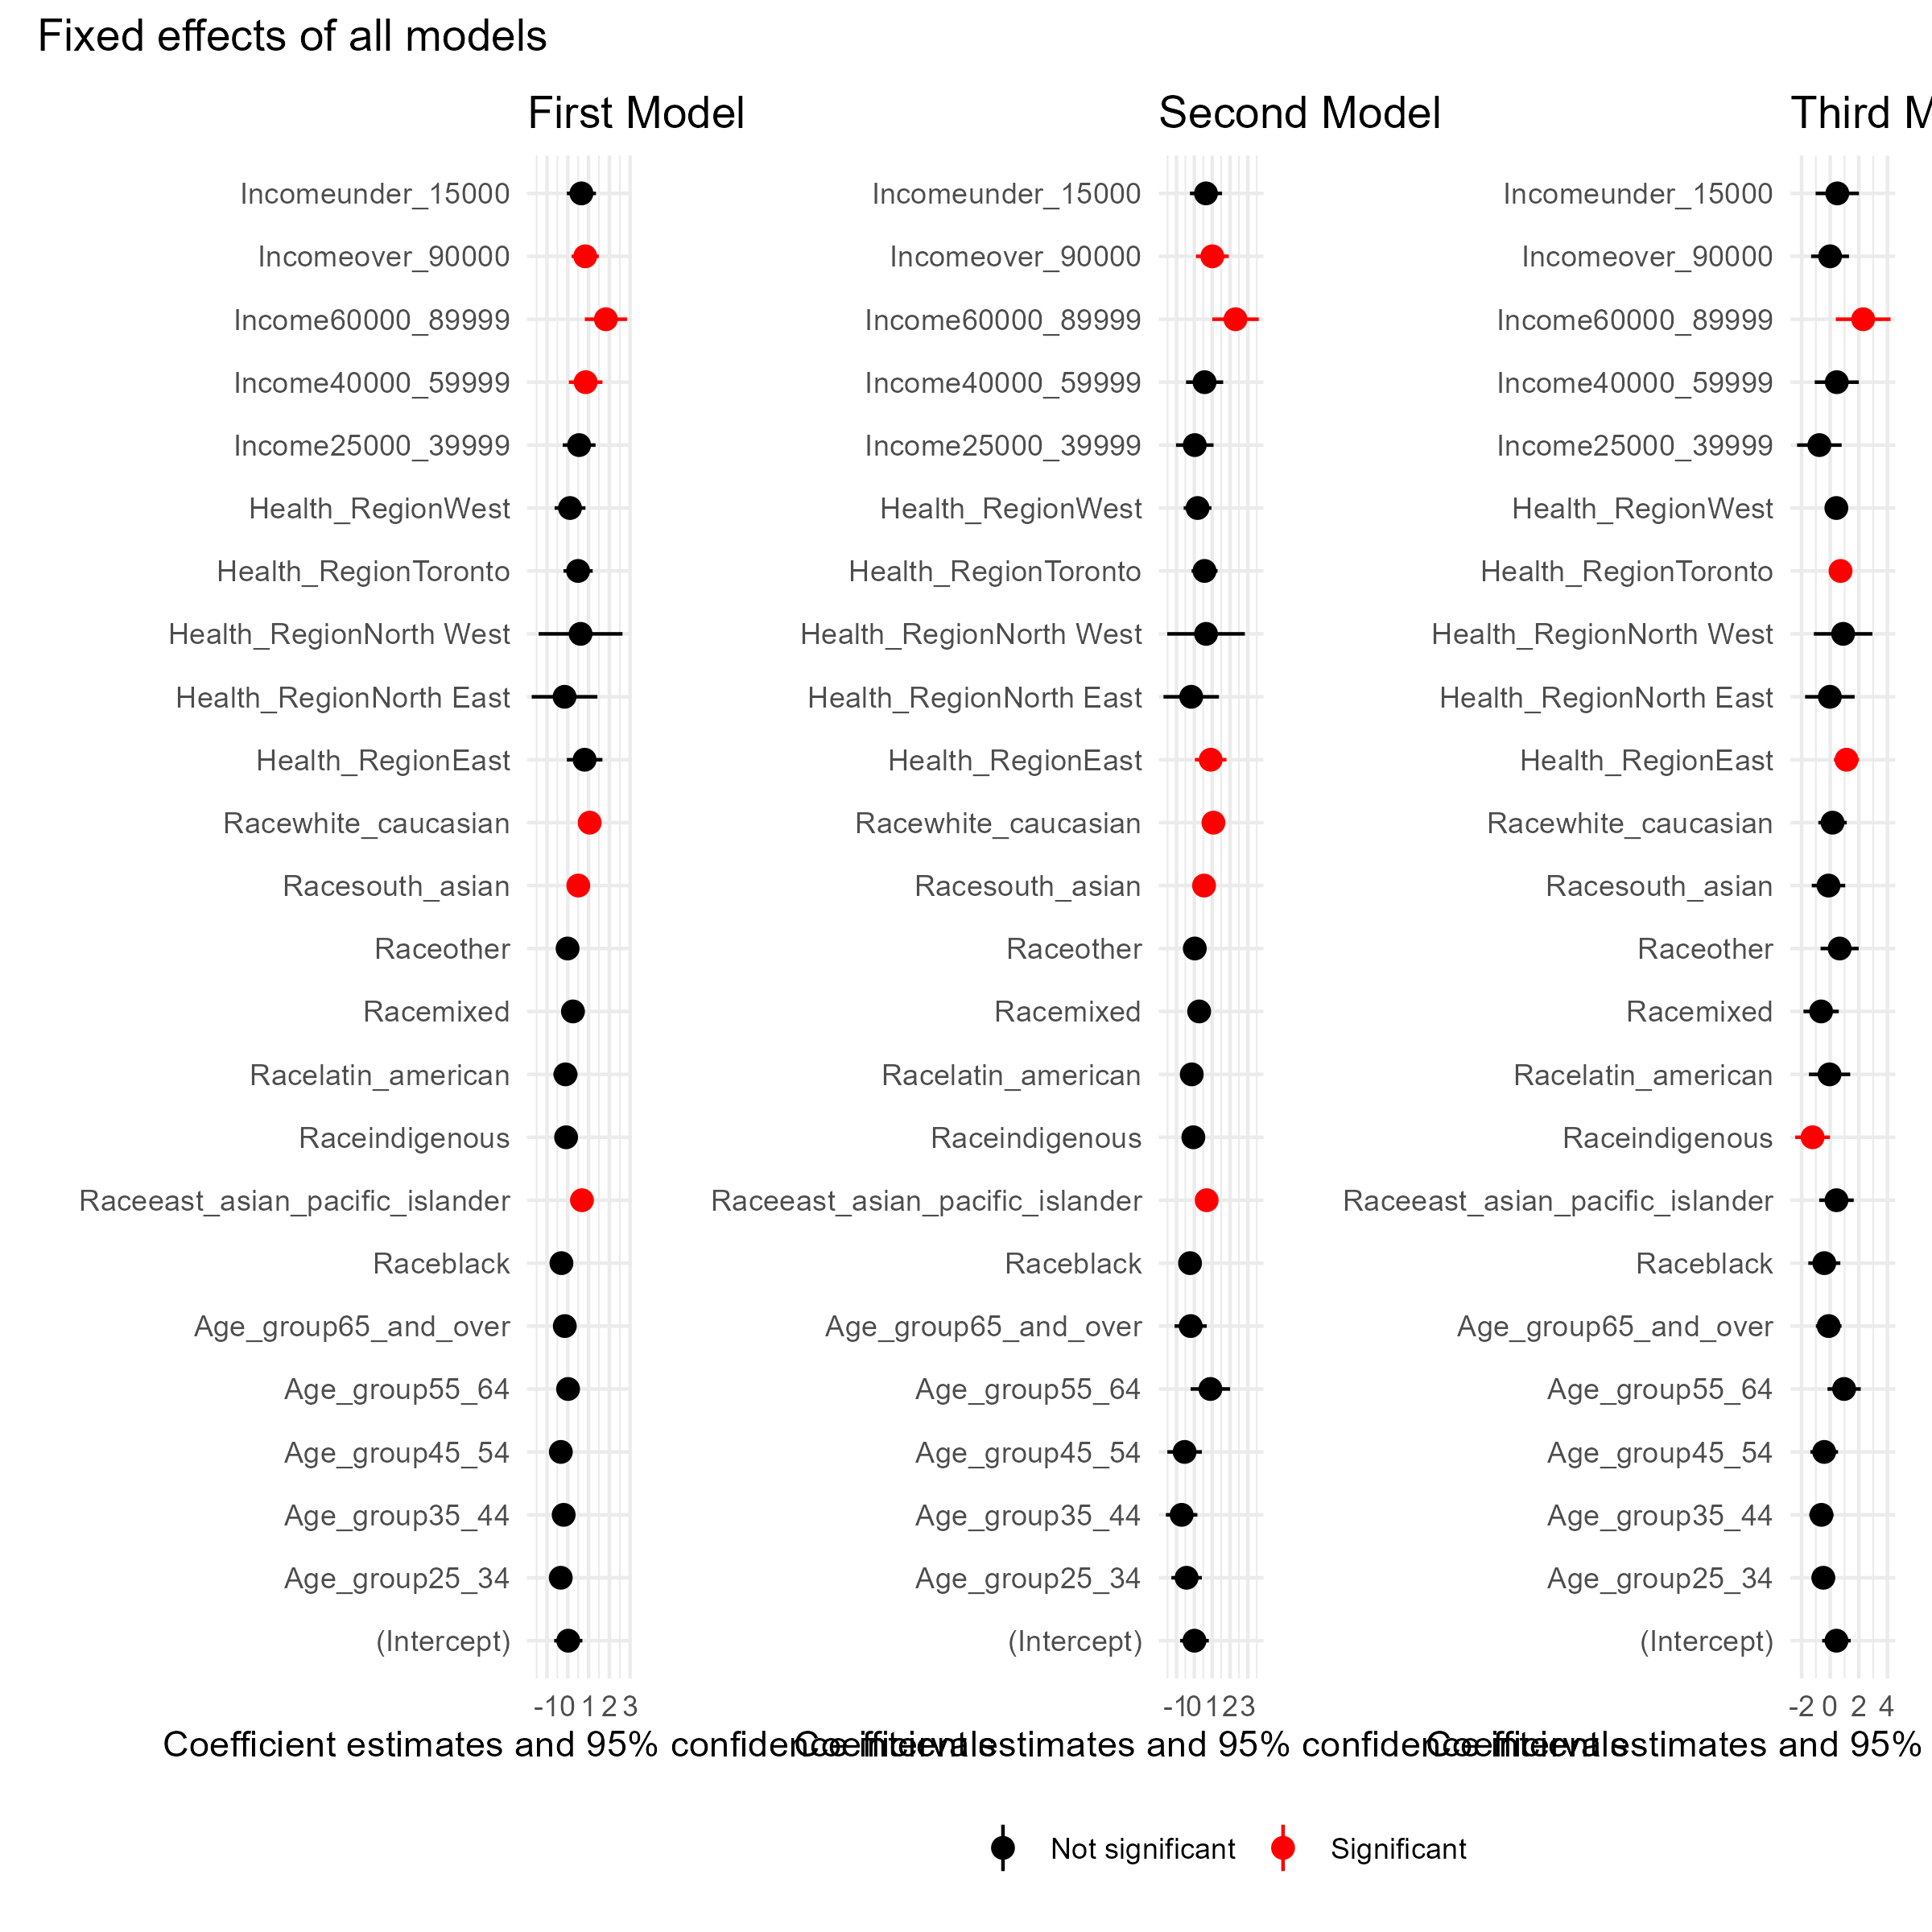
\includegraphics{Background_and_methods_Jan_12_files/figure-pdf/model-table-1.png}

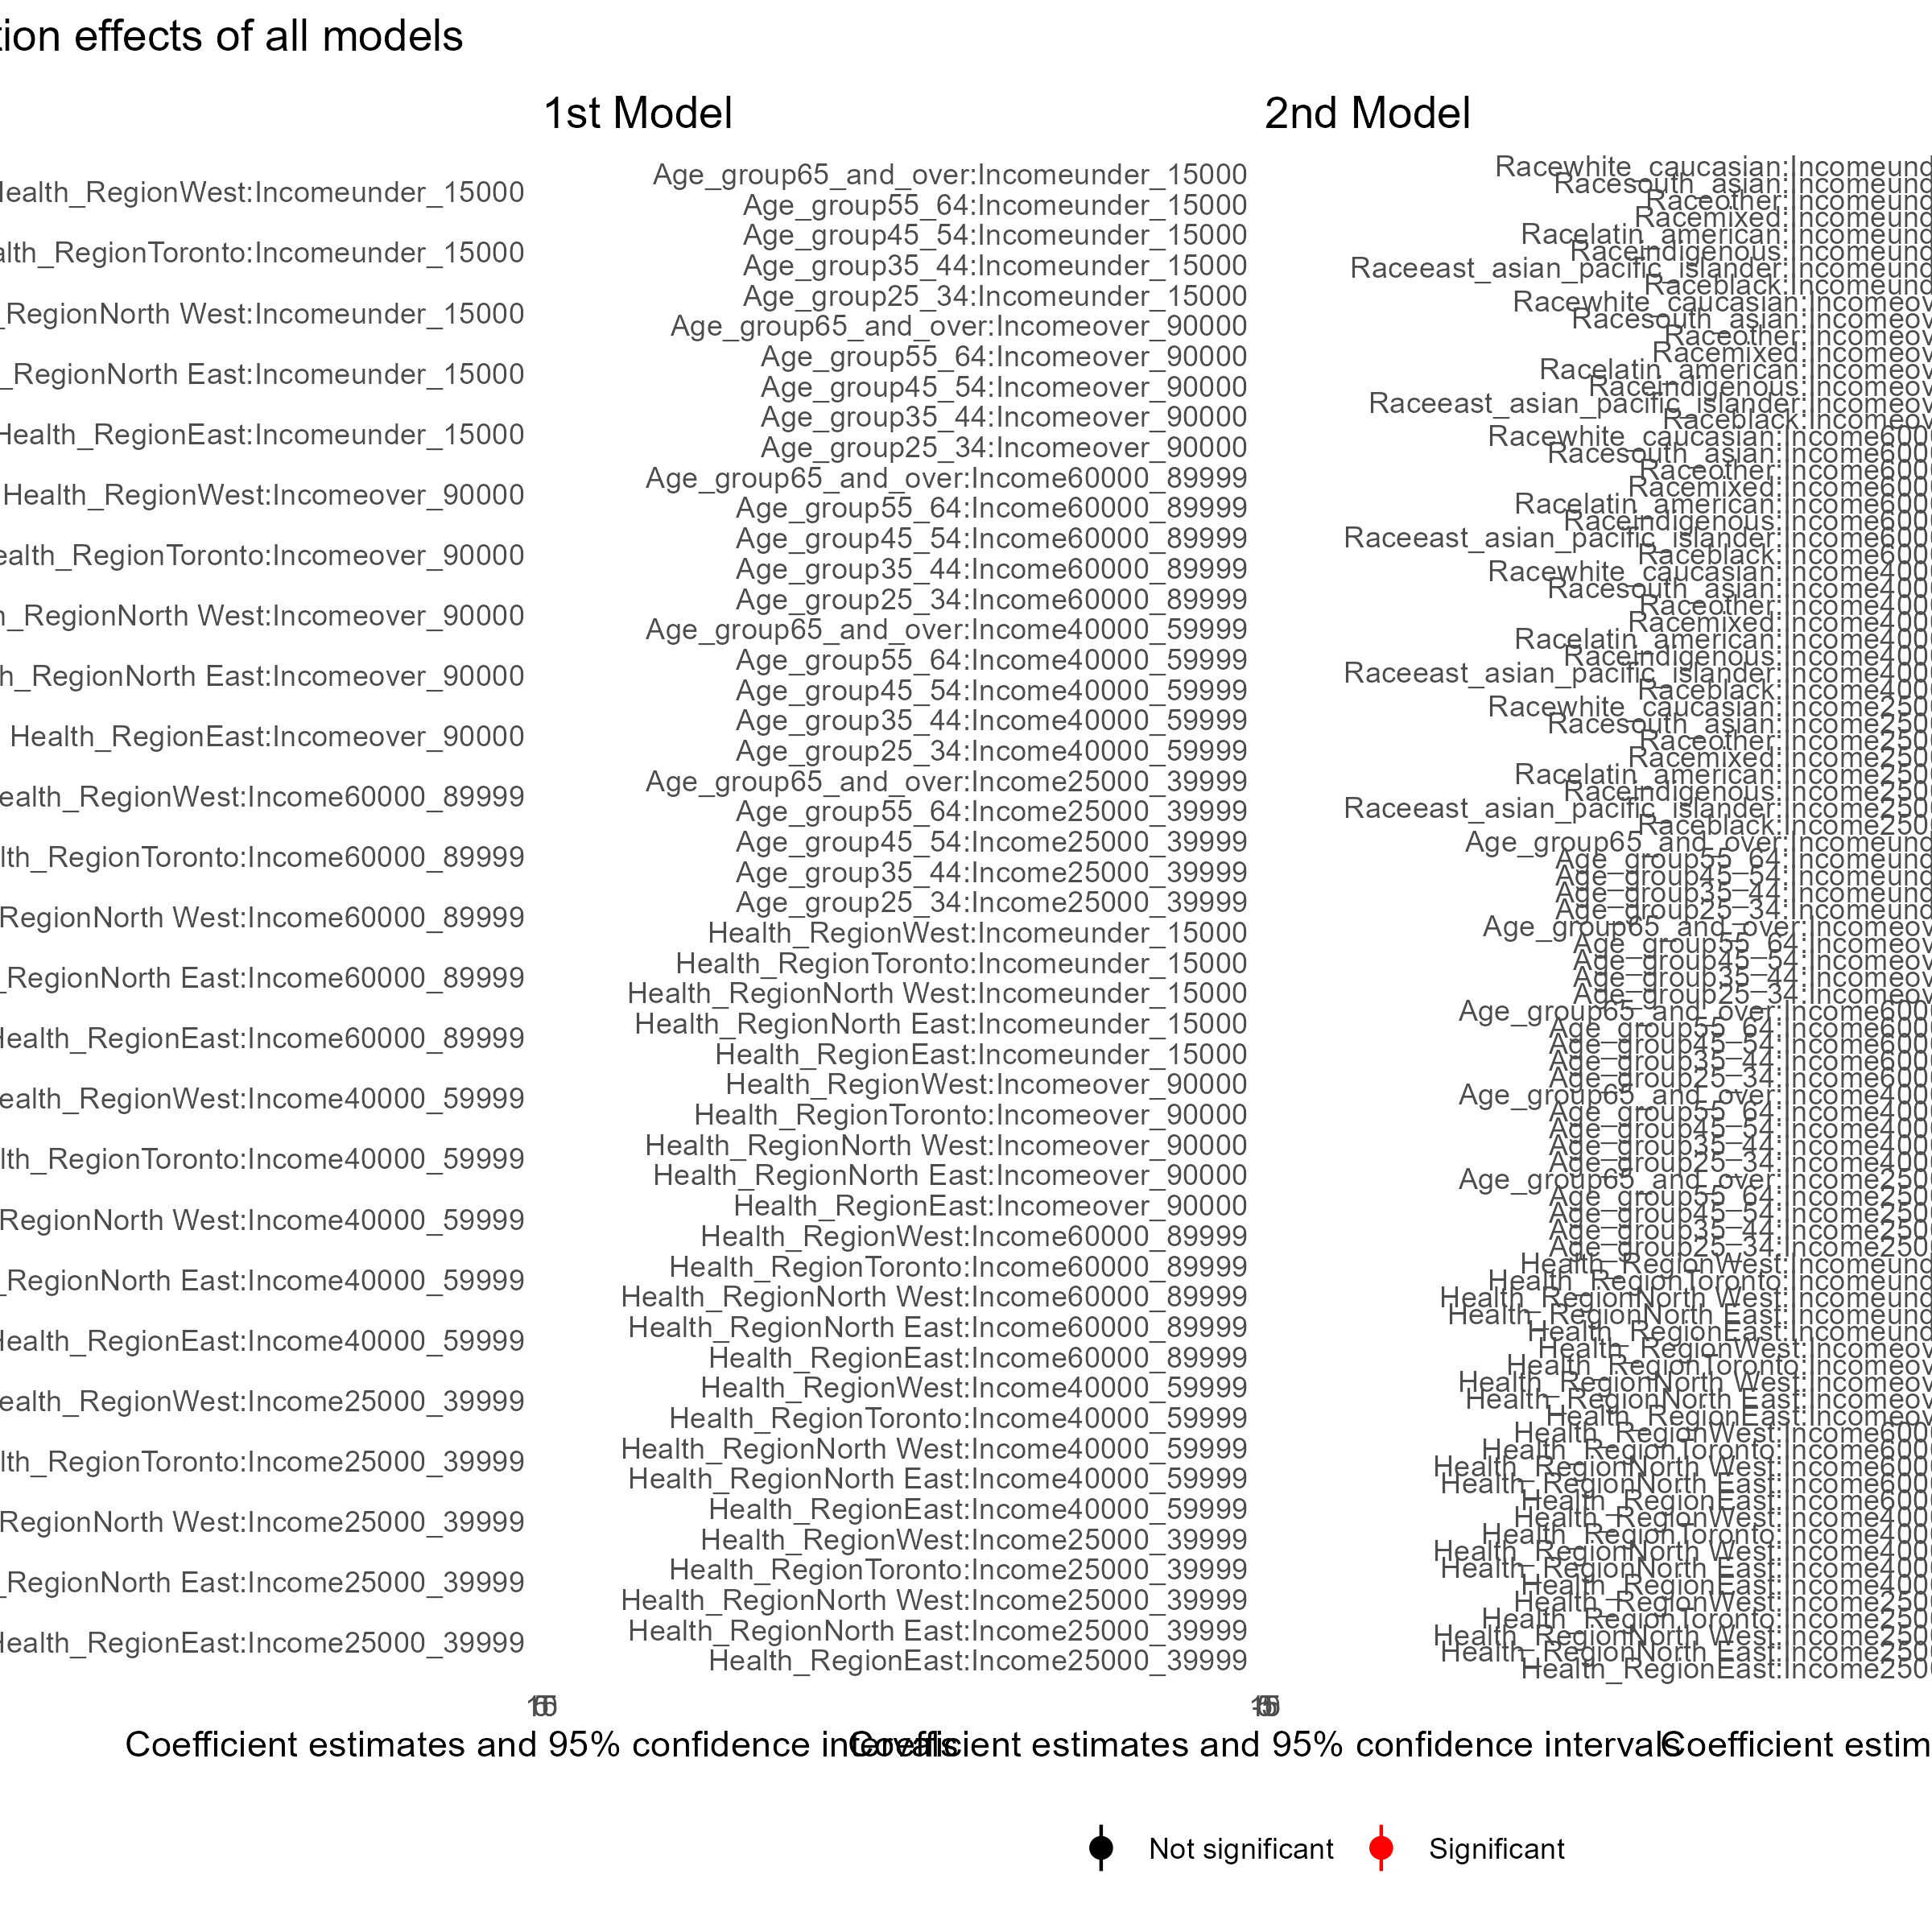
\includegraphics{Background_and_methods_Jan_12_files/figure-pdf/model-table-2.png}

\FloatBarrier

\hypertarget{references}{%
\subsection{References}\label{references}}

\hypertarget{refs}{}
\begin{CSLReferences}{0}{0}
\leavevmode\vadjust pre{\hypertarget{ref-WHO-Covid}{}}%
\CSLLeftMargin{1. }%
\CSLRightInline{{World Health Organization Coronavirus (COVID-19)
Dashboard}. Accessed November 27, 2022. \url{https://covid19.who.int/}}

\leavevmode\vadjust pre{\hypertarget{ref-tanne2020}{}}%
\CSLLeftMargin{2. }%
\CSLRightInline{Tanne JH. Covid-19: {FDA} panel votes to authorise
pfizer {BioNTech} vaccine. \emph{{BMJ}}. Published online December
2020:m4799.
doi:\href{https://doi.org/10.1136/bmj.m4799}{10.1136/bmj.m4799}}

\leavevmode\vadjust pre{\hypertarget{ref-bogoch2022}{}}%
\CSLLeftMargin{3. }%
\CSLRightInline{Bogoch II, Halani S. {COVID}-19 vaccines: A geographic,
social and policy view of vaccination efforts in ontario, canada.
\emph{Cambridge Journal of Regions, Economy and Society}. Published
online November 2022.
doi:\href{https://doi.org/10.1093/cjres/rsac043}{10.1093/cjres/rsac043}}

\leavevmode\vadjust pre{\hypertarget{ref-watson2022}{}}%
\CSLLeftMargin{4. }%
\CSLRightInline{Watson OJ, Barnsley G, Toor J, Hogan AB, Winskill P,
Ghani AC. Global impact of the first year of {COVID}-19 vaccination: A
mathematical modelling study. \emph{The Lancet Infectious Diseases}.
2022;22(9):1293-1302.
doi:\href{https://doi.org/10.1016/s1473-3099(22)00320-6}{10.1016/s1473-3099(22)00320-6}}

\leavevmode\vadjust pre{\hypertarget{ref-gerretsen2021}{}}%
\CSLLeftMargin{5. }%
\CSLRightInline{Gerretsen P, Kim J, Caravaggio F, et al. Individual
determinants of {COVID}-19 vaccine hesitancy. Inbaraj LR, ed.
\emph{{PLOS} {ONE}}. 2021;16(11):e0258462.
doi:\href{https://doi.org/10.1371/journal.pone.0258462}{10.1371/journal.pone.0258462}}

\leavevmode\vadjust pre{\hypertarget{ref-nafilyan2021}{}}%
\CSLLeftMargin{6. }%
\CSLRightInline{Nafilyan V, Dolby T, Razieh C, et al. Sociodemographic
inequality in {COVID}-19 vaccination coverage among elderly adults in
england: A national linked data study. \emph{{BMJ} Open}.
2021;11(7):e053402.
doi:\href{https://doi.org/10.1136/bmjopen-2021-053402}{10.1136/bmjopen-2021-053402}}

\leavevmode\vadjust pre{\hypertarget{ref-malik2020}{}}%
\CSLLeftMargin{7. }%
\CSLRightInline{Malik AA, McFadden SM, Elharake J, Omer SB. Determinants
of {COVID}-19 vaccine acceptance in the {US}.
\emph{{EClinicalMedicine}}. 2020;26:100495.
doi:\href{https://doi.org/10.1016/j.eclinm.2020.100495}{10.1016/j.eclinm.2020.100495}}

\leavevmode\vadjust pre{\hypertarget{ref-guay2022}{}}%
\CSLLeftMargin{8. }%
\CSLRightInline{Guay M, Maquiling A, Chen R, et al. Measuring
inequalities in {COVID}-19 vaccination uptake and intent: Results from
the canadian community health survey 2021. \emph{{BMC} Public Health}.
2022;22(1).
doi:\href{https://doi.org/10.1186/s12889-022-14090-z}{10.1186/s12889-022-14090-z}}

\leavevmode\vadjust pre{\hypertarget{ref-muhajarine2021}{}}%
\CSLLeftMargin{9. }%
\CSLRightInline{Muhajarine N, Adeyinka DA, McCutcheon J, Green KL,
Fahlman M, Kallio N. {COVID}-19 vaccine hesitancy and refusal and
associated factors in an adult population in saskatchewan, canada:
Evidence from predictive modelling. Gesser-Edelsburg A, ed. \emph{{PLOS}
{ONE}}. 2021;16(11):e0259513.
doi:\href{https://doi.org/10.1371/journal.pone.0259513}{10.1371/journal.pone.0259513}}

\leavevmode\vadjust pre{\hypertarget{ref-carter2022}{}}%
\CSLLeftMargin{10. }%
\CSLRightInline{Carter MA, Biro S, Maier A, Shingler C, Guan TH.
{COVID}-19 vaccine uptake in southeastern ontario, canada: Monitoring
and addressing health inequities. \emph{Journal of Public Health
Management and Practice}. 2022;28(6):615-623.
doi:\href{https://doi.org/10.1097/phh.0000000000001565}{10.1097/phh.0000000000001565}}

\leavevmode\vadjust pre{\hypertarget{ref-nguyen2021}{}}%
\CSLLeftMargin{11. }%
\CSLRightInline{Nguyen KH, Nguyen K, Corlin L, Allen JD, Chung M.
Changes in {COVID}-19 vaccination receipt and intention to vaccinate by
socioeconomic characteristics and geographic area, united states,
january 6 {\textendash} march 29, 2021. \emph{Annals of Medicine}.
2021;53(1):1419-1428.
doi:\href{https://doi.org/10.1080/07853890.2021.1957998}{10.1080/07853890.2021.1957998}}

\leavevmode\vadjust pre{\hypertarget{ref-mollalo2021}{}}%
\CSLLeftMargin{12. }%
\CSLRightInline{Mollalo A, Tatar M. Spatial modeling of {COVID}-19
vaccine hesitancy in the united states. \emph{International Journal of
Environmental Research and Public Health}. 2021;18(18):9488.
doi:\href{https://doi.org/10.3390/ijerph18189488}{10.3390/ijerph18189488}}

\leavevmode\vadjust pre{\hypertarget{ref-yang2022}{}}%
\CSLLeftMargin{13. }%
\CSLRightInline{Yang TC, Matthews SA, Sun F. Multiscale dimensions of
spatial process: {COVID}-19 fully vaccinated rates in u.s. counties.
\emph{American Journal of Preventive Medicine}. 2022;63(6):954-961.
doi:\href{https://doi.org/10.1016/j.amepre.2022.06.006}{10.1016/j.amepre.2022.06.006}}

\leavevmode\vadjust pre{\hypertarget{ref-tiu2022}{}}%
\CSLLeftMargin{14. }%
\CSLRightInline{Tiu A, Susswein Z, Merritt A, Bansal S. Characterizing
the spatiotemporal heterogeneity of the {COVID}-19 vaccination
landscape. \emph{American Journal of Epidemiology}.
2022;191(10):1792-1802.
doi:\href{https://doi.org/10.1093/aje/kwac080}{10.1093/aje/kwac080}}

\leavevmode\vadjust pre{\hypertarget{ref-bhuiyan2022}{}}%
\CSLLeftMargin{15. }%
\CSLRightInline{Bhuiyan MAN, Davis TC, Arnold CL, et al. Using the
social vulnerability index to assess {COVID}-19 vaccine uptake in
louisiana. \emph{{GeoJournal}}. Published online December 2022.
doi:\href{https://doi.org/10.1007/s10708-022-10802-5}{10.1007/s10708-022-10802-5}}

\leavevmode\vadjust pre{\hypertarget{ref-wood2022}{}}%
\CSLLeftMargin{16. }%
\CSLRightInline{Wood AJ, MacKintosh AM, Stead M, Kao RR. Predicting
future spatial patterns in {COVID}-19 booster vaccine uptake. Published
online September 2022.
doi:\href{https://doi.org/10.1101/2022.08.30.22279415}{10.1101/2022.08.30.22279415}}

\leavevmode\vadjust pre{\hypertarget{ref-choi2021}{}}%
\CSLLeftMargin{17. }%
\CSLRightInline{Choi KH, Denice PA, Ramaj S. Vaccine and {COVID}-19
trajectories. \emph{Socius: Sociological Research for a Dynamic World}.
2021;7:237802312110529.
doi:\href{https://doi.org/10.1177/23780231211052946}{10.1177/23780231211052946}}

\leavevmode\vadjust pre{\hypertarget{ref-mckinnon2021}{}}%
\CSLLeftMargin{18. }%
\CSLRightInline{McKinnon B, Quach C, Dubé Ève, Nguyen CT, Zinszer K.
Social inequalities in {COVID}-19 vaccine acceptance and uptake for
children and adolescents in montreal, canada. \emph{Vaccine}.
2021;39(49):7140-7145.
doi:\href{https://doi.org/10.1016/j.vaccine.2021.10.077}{10.1016/j.vaccine.2021.10.077}}

\leavevmode\vadjust pre{\hypertarget{ref-hussain2022}{}}%
\CSLLeftMargin{19. }%
\CSLRightInline{Hussain B, Latif A, Timmons S, Nkhoma K, Nellums LB.
Overcoming {COVID}-19 vaccine hesitancy among ethnic minorities: A
systematic review of {UK} studies. \emph{Vaccine}.
2022;40(25):3413-3432.
doi:\href{https://doi.org/10.1016/j.vaccine.2022.04.030}{10.1016/j.vaccine.2022.04.030}}

\leavevmode\vadjust pre{\hypertarget{ref-sargent2022}{}}%
\CSLLeftMargin{20. }%
\CSLRightInline{Sargent RH, Laurie S, Weakland LF, et al. Use of random
domain intercept technology to track {COVID}-19 vaccination rates in
real time across the united states: Survey study. \emph{Journal of
Medical Internet Research}. 2022;24(7):e37920.
doi:\href{https://doi.org/10.2196/37920}{10.2196/37920}}

\leavevmode\vadjust pre{\hypertarget{ref-deming1940}{}}%
\CSLLeftMargin{21. }%
\CSLRightInline{Deming WE, Stephan FF. On a least squares adjustment of
a sampled frequency table when the expected marginal totals are known.
\emph{The Annals of Mathematical Statistics}. 1940;11(4):427-444.
doi:\href{https://doi.org/10.1214/aoms/1177731829}{10.1214/aoms/1177731829}}

\leavevmode\vadjust pre{\hypertarget{ref-nguyen2022}{}}%
\CSLLeftMargin{22. }%
\CSLRightInline{Nguyen KH, Anneser E, Toppo A, Allen JD, Parott JS,
Corlin L. Disparities in national and state estimates of {COVID}-19
vaccination receipt and intent to vaccinate by race/ethnicity, income,
and age group among adults~\(\geq\)~18~years, united states.
\emph{Vaccine}. 2022;40(1):107-113.
doi:\href{https://doi.org/10.1016/j.vaccine.2021.11.040}{10.1016/j.vaccine.2021.11.040}}

\leavevmode\vadjust pre{\hypertarget{ref-shih2021}{}}%
\CSLLeftMargin{23. }%
\CSLRightInline{Shih SF, Wagner AL, Masters NB, Prosser LA, Lu Y,
Zikmund-Fisher BJ. Vaccine hesitancy and rejection of a vaccine for the
novel coronavirus in the united states. \emph{Frontiers in Immunology}.
2021;12.
doi:\href{https://doi.org/10.3389/fimmu.2021.558270}{10.3389/fimmu.2021.558270}}

\leavevmode\vadjust pre{\hypertarget{ref-cnat2022a}{}}%
\CSLLeftMargin{24. }%
\CSLRightInline{Cénat JM, Noorishad PG, Farahi SMMM, et al. Prevalence
and factors related to {COVID}-19 vaccine hesitancy and unwillingness in
canada: A systematic review and meta-analysis. \emph{Journal of Medical
Virology}. 2022;95(1).
doi:\href{https://doi.org/10.1002/jmv.28156}{10.1002/jmv.28156}}

\leavevmode\vadjust pre{\hypertarget{ref-cnat2022b}{}}%
\CSLLeftMargin{25. }%
\CSLRightInline{Cénat JM, Noorishad PG, Bakombo SM, et al. A systematic
review on vaccine hesitancy in black communities in canada: Critical
issues and research failures. \emph{Vaccines}. 2022;10(11):1937.
doi:\href{https://doi.org/10.3390/vaccines10111937}{10.3390/vaccines10111937}}

\leavevmode\vadjust pre{\hypertarget{ref-marchand2020}{}}%
\CSLLeftMargin{26. }%
\CSLRightInline{Marchand Y, Dubé J, Breau S. Exploring the causes and
consequences of regional income inequality in canada. \emph{Economic
Geography}. 2020;96(2):83-107.
doi:\href{https://doi.org/10.1080/00130095.2020.1715793}{10.1080/00130095.2020.1715793}}

\end{CSLReferences}



\end{document}
